\documentclass{beamer}

\mode<presentation>
{
  \usetheme{Boadilla}
  % or ...

  \setbeamercovered{transparent}
  % or whatever (possibly just delete it)
}


\title[Tupelo] % (optional, use only with long paper titles)
{Tupelo --- Towards Automated Disk Forensics}

%\subtitle
%{Sub} % (optional)

\author[] % (optional, use only with lots of authors)
{Stuart Maclean \\
University of Washington}
% - Use the \inst{?} command only if the authors have different
%   affiliation.

\date[] % (optional)
{Dec 2014}


\usepackage{graphicx}
%\usepackage{pbox}
\usepackage{tikz}


\begin{document}

%\includeonlyframes{current}

\begin{frame}
  \titlepage
\end{frame}


%\begin{frame}{Outline}
%  \tableofcontents[pausesections]
%  % You might wish to add the option [pausesections]
%\end{frame}

%%%%%%%%%%%%%%%%%%%%%%%%%%% %%%%%%%%%%%%%%%%%%%%%%%% %%%%%%%%%%%%%%%%%%%%%%%

\begin{frame}{Tupelo - What Is It?}

\begin{itemize}
\item Tupelo is a set of Java/C programs for efficient whole disk
  acquisition, storage and analysis.

\item Leverages existing open-source forensics library called
  Sleuthkit to walk filesystems.

\item Integrates with emerging standard STIX (Structured
  Threat Information Expression) to ingest and
  author shared information about malicious artifacts.

\end{itemize}

\end{frame}

%%%%%%%%%%%%%%%%%%%%%%%%%%%%%%%%%%%%%%%%%%%%%%%%%%%%%%%%%%%%%%%%%%%%%%%%%%%%


\begin{frame}{Tupelo Goals}

To minimize the time, effort and expense of maintaining the health of
computer hard drives.  To achieve this

\begin{itemize}

\item Whole drive acquisition must be easy and (relatively!) fast.

\item Repeated acquisition must be space-efficient.

\item Analysis of disk contents must be automated to the greatest
  extent possible.

\end{itemize}

\end{frame}

%%%%%%%%%%%%%%%%%%%%%%%%%%%%%%%%%%%%%%%%%%%%%%%%%%%%%%%%%%%%%%%%%%%%%%%%%%%%

\begin{frame}{The Problem of Trust}

If the drive you wish to acquire is suspected of containing
malicious artifacts, how can software residing on that same disk
be relied upon to present accurate disk content? 

\vskip 20pt

Tupelo does ``dead disk acquisition'', and runs from trusted media,
e.g. a bootable CD/USB.  Yes, you have to power down.

\end{frame}

%%%%%%%%%%%%%%%%%%%%%%%%%%%%%%%%%%%%%%%%%%%%%%%%%%%%%%%%%%%%%%%%%%%%%%%%%%%%

\begin{frame}{Tupelo Workflows and the Store}

\begin{itemize}
\item
Users acquire whole drive contents, storing a copy in a {\em Tupelo
  store}.

\item
Data transitions from being {\em unmanaged} to being {\em managed}.

\item
Once managed, contents are analysed: filesystems, un-allocated
areas.

\item
Analysis results also placed in the store alongside the managed data
as {\em attributes}, key/value pairs with arbitrary values.

\item
Same disk can be acquired repeatedly, and many disks can be acquired.

\end{itemize}

Store is essentially a structured (but not relational) database.

\end{frame}

%%%%%%%%%%%%%%%%%%%%%%%%%%%%%%%%%%%%%%%%%%%%%%%%%%%%%%%%%%%%%%%%%%%%%%%%%%

\begin{frame}{Analysis Products}

For each managed disk (what/when), run store tools (via Sleuthkit)

\begin{itemize}
\item Un-allocated areas hash - finds MBR malware, hidden data.

\item
Filesystem hashes - input to IOC-based lookup.

\item
Bodyfiles - expanded hashes, contain file times, owner etc.

\end{itemize}

Examples?

\end{frame}

%%%%%%%%%%%%%%%%%%%%%%%%%%%%%%%%%%%%%%%%%%%%%%%%%%%%%%%%%%%%%%%%%%%%%%%

\begin{frame}{Supported Disk Types}

Can acquire three flavors of whole disk content:

\begin{description}
\item[Physical] Entire hard drive.  To ensure ``dead'', boot from
  Tupelo CD.

\item[Virtual] Hard drive of a virtual machine.  To ensure ``dead'',
  acquire with VM powered off.  VirtualBox and VMWare disks supported.

\item[Disk Image] A previously obtained whole disk image, as a file.
  Dead by definition.
\end{description}

Could also boot virtual machines from virtualized Tupelo CD, then 
a virtual disk is essentially physical.

\end{frame}

%%%%%%%%%%%%%%%%%%%%%%%%%%%%%%%%%%%%%%%%%%%%%%%%%%%%%%%%%%%%%%%%%%%%%%%

\begin{frame}[fragile]{What and When}

Everything submitted to the Tupelo store is tagged with two
identifying labels.

\begin{description}
\item[What]  An identifier for the disk.  We use the disk's vendor
  plus serial number, not any info stored {\em on} the disk, nor any
  local user name for the data.  

\item[When] A timestamp, in the form of a sessionID (ticket,token)
  handed out by the store when the client connects.  Store ensures
  unique and serialized distribution of sessionIDs.
\end{description}

Example:
\begin{verbatim}
what = ATA-SAMSUNG HD253GJ-S26CJ90B203913
when = 20150106.0005
\end{verbatim}

\end{frame}

%%%%%%%%%%%%%%%%%%%%%%%%%%%%%%%%%%%%%%%%%%%%%%%%%%%%%%%%%%%%%%%%%%%%%%%

\begin{frame}{Use Cases}

Tupelo's generality supports several modes of use:

\begin{itemize}
\item 
Single User

\item
Local Area Administrator

\item
Wide Area Administrator 

\end{itemize}

\end{frame}


%%%%%%%%%%%%%%%%%%%%%%%%%%%%%%%%%%%%%%%%%%%%%%%%%%%%%%%%%%%%%%%%%%%%%%

\begin{frame}{Single User}

\begin{itemize}
\item Home user, one system, one hard drive.

\item Store is an external hard disk (USB/eSATA)

\item Acquire on a schedule, e.g. once a week.

\item Run store tools manually to produce volume, filesystem
  differences.

\item Useful as a backup?

\end{itemize}

\end{frame}

%%%%%%%%%%%%%%%%%%%%%%%%%%%%%%%%%%%%%%%%%%%%%%%%%%%%%%%%%%%%%%%%%%%%%%

\begin{frame}{Local Area Administrator}

\begin{itemize}
\item Group administrator.  Many drives to acquire, also on a
  schedule.  Possible end-user does the acquire!

\item Store is network-accessible.

\item Reference images (e.g. vanilla Win7 install) added to
  store reduces time spent classifying artifacts.  

\item
Also store known goods (e.g. NSRL) and known bads (e.g. IOCs)

\end{itemize}
\end{frame}

%%%%%%%%%%%%%%%%%%%%%%%%%%%%%%%%%%%%%%%%%%%%%%%%%%%%%%%%%%%%%%%%%%%%%%

\begin{frame}{Wide Area Administrator}

In addition to local area administrator usage

\begin{itemize}
\item
Stores linked to form a graph, expands knowledge base.

\item
Stores listen on message bus for IOCs (e.g. STIX).  Enables near
real-time identification of malicious artifacts.

\end{itemize}

\end{frame}

%%%%%%%%%%%%%%%%%%%%%%%%%%%%%%%%%%%%%%%%%%%%%%%%%%%%%%%%%%%%%%%%%%%%%%%%%%%%

\begin{frame}{Message Bus Framework}

In addition to accepting unmanaged data, over e.g. http, Tupelo store
also listens on a message bus (currently AMQP):

\begin{itemize}
\item
Client programs ask (via AMQP posts) ``Who has seen this hash?''.

\item
Results relayed to requester, but also to originating Tupelo user.

\item
Frees Tupelo user from drudgery of IOC handling.

\end{itemize}

\end{frame}


%%%%%%%%%%%%%%%%%%%%%%%%%%% %%%%%%%%%%%%%%%%%%%%%%%% %%%%%%%%%%%%%%%%%%%%%%%

\begin{frame}{Tupelo System Architecture}

\begin{center}
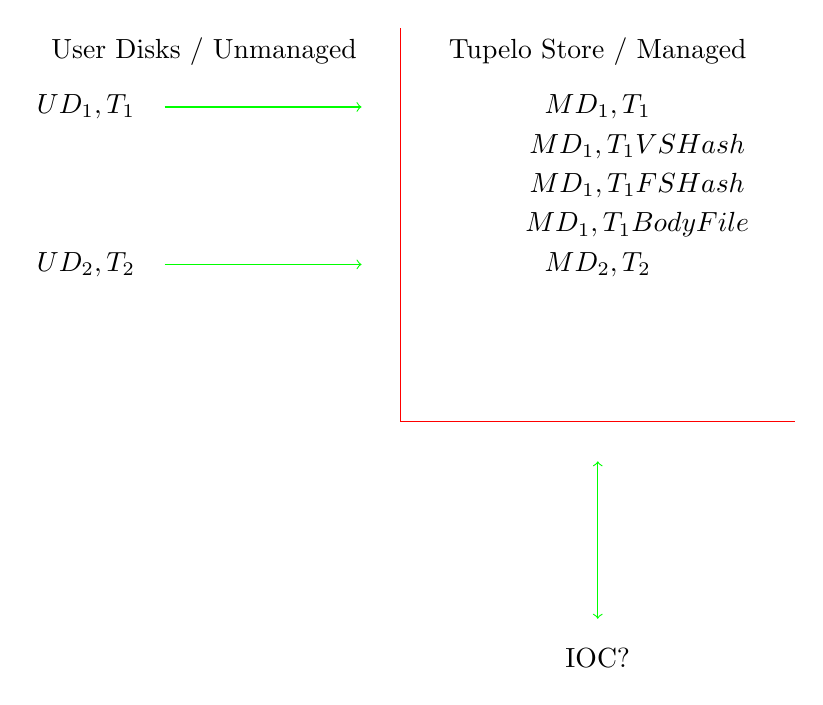
\begin{tikzpicture}

%\draw[help lines] (0,0) grid (10,10);

\draw [red] (5,5) -- (5,10);
\draw [red] (5,5) -- (10,5);
\node [below] at (2.5,10) {User Disks / Unmanaged};
\node [below] at (7.5,10) {Tupelo Store / Managed};

%% First putdata, user 1
\draw [->, green] (2,9) -- (4.5,9);
\node at (1,9) { $UD_{1},T_{1}$ };
\node at (7.5,9) { $MD_{1},T_{1}$ };
\node at (8,8.5) { $MD_{1},T_{1} VSHash$ };
\node at (8,8) { $MD_{1},T_{1} FSHash$ };
\node at (8,7.5) { $MD_{1},T_{1} BodyFile$ };

%% First putdata, user 2
\draw [->, green] (2,7) -- (4.5,7);
\node at (1,7) { $UD_{2},T_{2}$ };
\node at (7.5,7) { $MD_{2},T_{2}$ };

%% AMQP
\draw [<->, green] (7.5,4.5) -- (7.5,2.5);
\node at (7.5,2) { IOC?};

\end{tikzpicture}
\end{center}

\end{frame}



\begin{frame}{Initial Data Acquisition}

\begin{center}
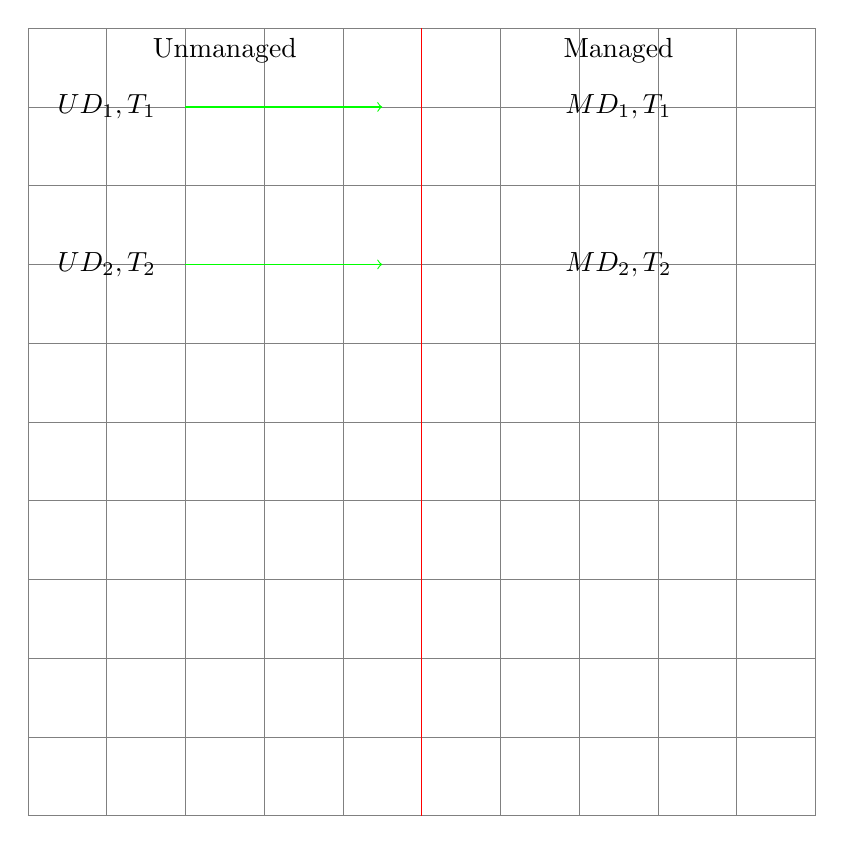
\begin{tikzpicture}

\draw[help lines] (0,0) grid (10,10);

\draw [red] (5,0) -- (5,10);
\node [below] at (2.5,10) {Unmanaged};
\node [below] at (7.5,10) {Managed};

%% First putdata, user 1
\draw [->, green] (2,9) -- (4.5,9);
\node at (1,9) { $UD_{1},T_{1}$ };
\node at (7.5,9) { $MD_{1},T_{1}$ };

%% First putdata, user 2
\draw [->, green] (2,7) -- (4.5,7);
\node at (1,7) { $UD_{2},T_{2}$ };
\node at (7.5,7) { $MD_{2},T_{2}$ };

\end{tikzpicture}
\end{center}

\end{frame}

%%%%%%%%%%%%%%%%%%%%%%%%%%%%%%%%%%%%%%%%%%%%%%%%%%%%%%%%%%%%%%%%%%%%%%%%%%%%

\begin{frame}{Subsequent Data Acquisition}

\begin{center}
\begin{tikzpicture}

%\draw[help lines] (0,0) grid (10,8);

%% Existing putdata
\draw [->] (1,1) -- (4,4);
\node [below] at (1,1) { $UD_{1},T_{1}$ };

%% Second putdata
\draw [->] (3,0.5) -- (4.5,4);
\node [below] at (3,0.5) { $UD_{1},T_{3}$ };

\draw (4,4) rectangle (6,6);

%% Existing putdata
\draw [->] (9,1) -- (6,4);
\node [below] at (9,1) { $UD_{2},T_{2}$ };

%% Second putdata
\draw [->] (7,0.5) -- (5.5,4);
\node [below] at (7,0.5) { $UD_{2},T_{4}$ };

\end{tikzpicture}
\end{center}

\end{frame}

%%%%%%%%%%%%%%%%%%%%%%%%%%%%%%%%%%%%%%%%%%%%%%%%%%%%%%%%%%%%%%%%%%%%%%%%%%%%

\begin{frame}{Stored Attributes Accompany Data}

\begin{center}
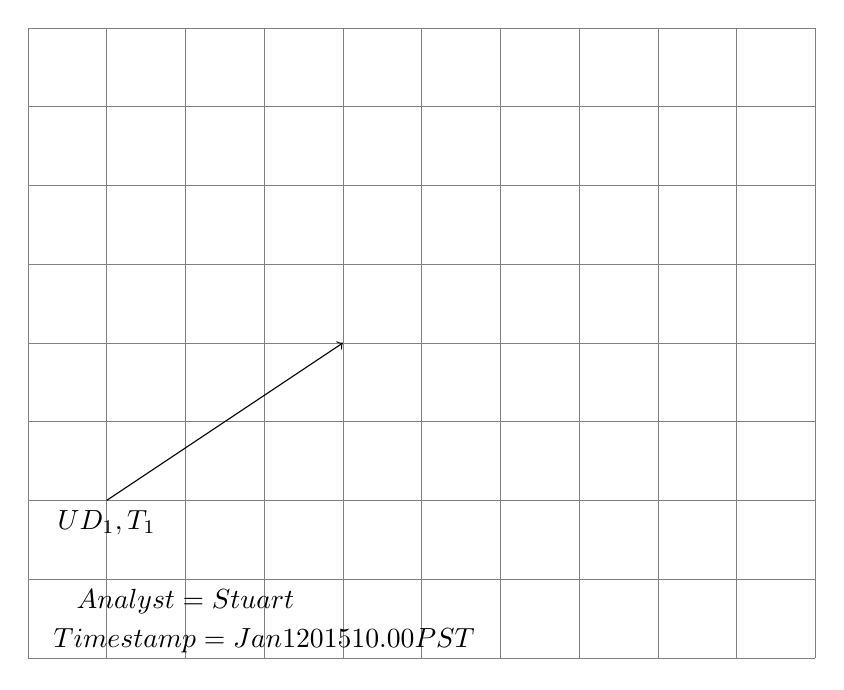
\begin{tikzpicture}

\draw[help lines] (0,0) grid (10,8);

%% Existing putdata
\draw [->] (1,2) -- (4,4);
\node [below] at (1,2) { $UD_{1},T_{1}$ };

%% Attach attributes
\node [below] at (2,1) { $Analyst = Stuart$ };
\node [below] at (3,0.5) { $Timestamp = Jan 1 2015 10.00 PST$ };

\end{tikzpicture}
\end{center}

\end{frame}


\end{document}

% eof
